% ========================================
%	Header einbinden
% ========================================

\documentclass[bibtotoc,titlepage]{scrartcl}

% Deutsche Spracheinstellungen
\usepackage[ngerman,german]{babel, varioref}
\usepackage[T1]{fontenc}
\usepackage[utf8]{inputenc}

%\usepackage{marvosym}

\usepackage{amsfonts}
\usepackage{amssymb}
\usepackage{amsmath}
\usepackage{amscd}
\usepackage{amstext}
\usepackage{float}
\usepackage{caption}
\usepackage{wrapfig}
\usepackage{setspace}
\usepackage{threeparttable}
\usepackage{footnote}

\usepackage{caption}
\usepackage{subcaption}

\newfloat{formel}{htbp}{for}
\floatname{formel}{Formel}


\usepackage{longtable}

%\usepackage{bibgerm}

\usepackage{footnpag}

\usepackage{ifthen}                 %%% package for conditionals in TeX
\usepackage{siunitx}
%Fr textumflossene Bilder und Tablellen
%\usepackage{floatflt} - veraltet

%Fr Testzwecke aktivieren, zeigt labels und refs im Text an.
%\usepackage{showkeys}

% Abstand zwischen zwei Abs�zen nach DIN (1,5 Zeilen)
% \setlength{\parskip}{1.5ex plus0.5ex minus0.5ex}

% Einrckung am Anfang eines neuen Absatzes nach DIN (keine)
%\setlength{\parindent}{0pt}

% R�der definieren
% \setlength{\oddsidemargin}{0.3cm}
% \setlength{\textwidth}{15.6cm}

% bessere Bildunterschriften
%\usepackage[center]{caption2}


% Probleml�ungen beim Umgang mit Gleitumgebungen
\usepackage{float}

% Nummeriert bis zur Strukturstufe 3 (also <section>, <subsection> und <subsubsection>)
%\setcounter{secnumdepth}{3}

% Fhrt das Inhaltsverzeichnis bis zur Strukturstufe 3
%\setcounter{tocdepth}{3}

\usepackage{exscale}

\newenvironment{dsm} {\begin{displaymath}} {\end{displaymath}}
\newenvironment{vars} {\begin{center}\scriptsize} {\normalsize \end{center}}


\newcommand {\en} {\varepsilon_0}               % Epsilon-Null aus der Elektrodynamik
\newcommand {\lap} {\; \mathbf{\Delta}}         % Laplace-Operator
\newcommand {\R} { \mathbb{R} }                 % Menge der reellen Zahlen
\newcommand {\e} { \ \mathbf{e} }               % Eulersche Zahl
\renewcommand {\i} { \mathbf{i} }               % komplexe Zahl i
\newcommand {\N} { \mathbb{N} }                 % Menge der nat. Zahlen
\newcommand {\C} { \mathbb{C} }                 % Menge der kompl. Zahlen
\newcommand {\Z} { \mathbb{Z} }                 % Menge der kompl. Zahlen
\newcommand {\limi}[1]{\lim_{#1 \rightarrow \infty}} % Limes unendlich
\newcommand {\sumi}[1]{\sum_{#1=0}^\infty}
\newcommand {\rot} {\; \mathrm{rot} \,}         % Rotation
\newcommand {\grad} {\; \mathrm{grad} \,}       % Gradient
\newcommand {\dive} {\; \mathrm{div} \,}        % Divergenz
\newcommand {\dx} {\; \mathrm{d} }              % Differential d
\newcommand {\cotanh} {\; \mathrm{cotanh} \,}   %Cotangenshyperbolicus
\newcommand {\asinh} {\; \mathrm{areasinh} \,}  %Area-Sinus-Hyp.
\newcommand {\acosh} {\; \mathrm{areacosh} \,}  %Area-Cosinus-H.
\newcommand {\atanh} {\; \mathrm{areatanh} \,}  %Area Tangens-H.
\newcommand {\acoth} {\; \mathrm{areacoth} \,}  % Area-cotangens
\newcommand {\Sp} {\; \mathrm{Sp} \,}
\newcommand {\mbe} {\stackrel{\text{!}}{=}}     %Must Be Equal
\newcommand{\qed} { \hfill $\square$\\}
\renewcommand{\i} {\imath}
\def\captionsngerman{\def\figurename{\textbf{Abb.}}}

%%%%%%%%%%%%%%%%%%%%%%%%%%%%%%%%%%%%%%%%%%%%%%%%%%%%%%%%%%%%%%%%%%%%%%%%%%%%
% SWITCH FOR PDFLATEX or LATEX
%%%%%%%%%%%%%%%%%%%%%%%%%%%%%%%%%%%%%%%%%%%%%%%%%%%%%%%%%%%%%%%%%%%%%%%%%%%%
%%%
\ifx\pdfoutput\undefined %%%%%%%%%%%%%%%%%%%%%%%%%%%%%%%%%%%%%%%%% LATEX %%%
%%%
\usepackage[dvips]{graphicx}       %%% graphics for dvips
\DeclareGraphicsExtensions{.eps,.ps}   %%% standard extension for included graphics
\usepackage[ps2pdf]{thumbpdf}      %%% thumbnails for ps2pdf
\usepackage[ps2pdf,                %%% hyper-references for ps2pdf
bookmarks=true,%                   %%% generate bookmarks ...
bookmarksnumbered=true,%           %%% ... with numbers
hypertexnames=false,%              %%% needed for correct links to figures !!!
breaklinks=true,%                  %%% breaks lines, but links are very small
linkbordercolor={0 0 1},%          %%% blue frames around links
pdfborder={0 0 112.0}]{hyperref}%  %%% border-width of frames
%                                      will be multiplied with 0.009 by ps2pdf
%
%\hypersetup{ pdfauthor   = {Hannes Franke; Julius Tilly},
%pdftitle    = {x}, pdfsubject  = {Protokoll FP}, pdfkeywords = {V301, Innenwiderstand, Leistungsanpassung},
%pdfcreator  = {LaTeX with hyperref package}, pdfproducer = {dvips
%+ ps2pdf} }
%%%
\else %%%%%%%%%%%%%%%%%%%%%%%%%%%%%%%%%%%%%%%%%%%%%%%%%%%%%%%%%% PDFLATEX %%%
%%%
\usepackage[pdftex]{graphicx}      %%% graphics for pdfLaTeX
\DeclareGraphicsExtensions{.pdf}   %%% standard extension for included graphics
\usepackage[pdftex]{thumbpdf}      %%% thumbnails for pdflatex
\usepackage[pdftex,                %%% hyper-references for pdflatex
bookmarks=true,%                   %%% generate bookmarks ...
bookmarksnumbered=true,%           %%% ... with numbers
hypertexnames=false,%              %%% needed for correct links to figures !!!
breaklinks=true,%                  %%% break links if exceeding a single line
linkbordercolor={0 0 1},
linktocpage]{hyperref} %%% blue frames around links
%                                  %%% pdfborder={0 0 1} is the default
% \hypersetup{
% pdftitle    = {V301 Innenwiderstand und Leistungsanpassung}, 
% pdfsubject  = {Protokoll AP}, 
% pdfkeywords = {V301, Innenwiderstand, Leistungsanpassung},
% pdfsubject  = {Protokoll AP},
% pdfkeywords = {V301, Innenwiderstand, Leistungsanpassung}}
%                                  %%% pdfcreator, pdfproducer,
%                                      and CreationDate are automatically set
%                                      by pdflatex !!!
\pdfadjustspacing=1                %%% force LaTeX-like character spacing
\usepackage{epstopdf}
%
\fi %%%%%%%%%%%%%%%%%%%%%%%%%%%%%%%%%%%%%%%%%%%%%%%%%%% END OF CONDITION %%%
%%%%%%%%%%%%%%%%%%%%%%%%%%%%%%%%%%%%%%%%%%%%%%%%%%%%%%%%%%%%%%%%%%%%%%%%%%%%
% seitliche Tabellen und Abbildungen
%\usepackage{rotating}
\usepackage{ae}
\usepackage{
  array,
  booktabs,
  dcolumn
}
\makeatletter 
  \renewenvironment{figure}[1][] {% 
    \ifthenelse{\equal{#1}{}}{% 
      \@float{figure} 
    }{% 
      \@float{figure}[#1]% 
    }% 
    \centering 
  }{% 
    \end@float 
  } 
  \makeatother 


  \makeatletter 
  \renewenvironment{table}[1][] {% 
    \ifthenelse{\equal{#1}{}}{% 
      \@float{table} 
    }{% 
      \@float{table}[#1]% 
    }% 
    \centering 
  }{% 
    \end@float 
  } 
  \makeatother 
%\usepackage{listings}
%\lstloadlanguages{[Visual]Basic}
%\allowdisplaybreaks[1]
%\usepackage{hycap}
%\usepackage{fancyunits}
\usepackage{subcaption}
\usepackage{placeins}
\newcommand{\minwidth}{0.47}
\newcommand{\minwidththree}{0.49}


% ========================================
%	Angaben für das Titelblatt
% ========================================

\title{Search for $t\bar t$ Resonances with ATLAS data \\ \vspace{.5cm}% Titel des Versuchs 
	\large TU Dortmund, Fakultät Physik\\ 
	\normalsize Fortgeschrittenen-Praktikum}

\author{Dimitrios Skodras\\			% Name Praktikumspartner A
	{\small \href{dimitrios.skodras@tu-dortmund.de}{dimitrios.skodras@tu-dortmund.de}}	% Erzeugt interaktiven einen Link
				\and			% um einen weiteren Author hinzuzfügen
	Julius Tilly\\					% Name Praktikumspartner B
	{\small \href{julius.tilly@tu-dortmund.de}{julius.tilly@tu-dortmund.de}}		% Erzeugt interaktiven einen Link
}
\date{27.09.2016}				% Das Datum der Versuchsdurchführung

% ========================================
%	Das Dokument beginnt
% ========================================

\begin{document}
	
% ========================================
%	Titelblatt erzeugen
% ========================================

\maketitle					% Jetzt wird die Titelseite erzeugt
\thispagestyle{empty} 				% Weder Kopfzeile noch Fußzeile

% ========================================
%	Der Vorspann
% ========================================

%\newpage					% Wenn Verzeichnisse auf einer neuen Seite beginnen sollen
%\pagestyle{empty}				% Weder Kopf- noch Fußzeile für Verzeichnisse

\tableofcontents

%\newpage					% eine neue Seite
%\thispagestyle{empty}				% Weder Kopf- noch Fußzeile für Verzeichnisse
%\listoffigures					% Abbildungsverzeichnis

%\newpage					% eine neue Seite
%\thispagestyle{empty}				% Weder Kopf- noch Fußzeile für Verzeichnisse
%\listoftables					% Tabellenverzeichnis
\newpage					% eine neue Seite


% ========================================
%	Kapitel
% ========================================

\section{Introduction}
Besides its properties to have very accurate estimations for the processes it is applicable to, the Standard Model (SM) lacks the explanation for 
several phenomena. Many of them hint at the electroweak scale of order $\mathcal{O}$(100 GeV) where new physics is expected to occur. One new particle
proposed by some models beyond the SM is $Z'$. Its properties are very similar to the SM-$Z$ boson but is around an order of magnitude heavier so that
it can decay into a top-antitop pair $t\bar t$. It may furthermore serve as a mediator to a dark sector or may have flavour violating interactions, 
possibly 
explaining flavour anomalies in $B$-meson physics. Considerations as the latter two, however, are beyond the scope of this work. The top pair mainly
gets produced via the strong interaction of two gluons $g$ and decays weakly into two $b$-quarks and two $W$-bosons which themselves decay further 
expressed by three topologies (see Fig. \ref{pic:feynman}). 
\begin{figure}
 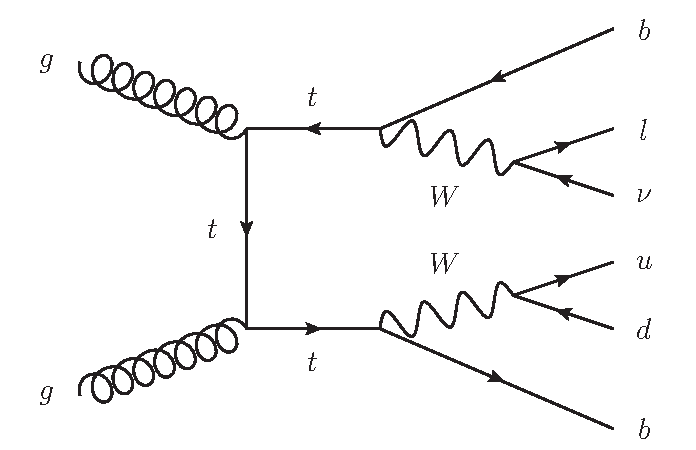
\includegraphics[width=0.5\textwidth]{../pics/e4.pdf}
 \caption{Most dominant process for creation and decay of a top pair at an hadron collider.}
 \label{pic:feynman}
\end{figure}
One may decay into a lepton pair and the other into a quark pair (i.e. lepton$+$jets) or both decay leptonically 
(i.e. dilepton) or hadronically (i.e. all hadron). Due to its color representation and the quark flavour violation, decays into quarks are much more 
probable compared to lepton involving ones. But they are more complicate to identify, i.e. reconstructed, as $t$ decay products as a result of 
confinement since jets can arise out of many other processes and the background in the hadronic channel is a lot bigger compared to the leptonic
channel. The tradeoff is therefore to focus on the lepton$+$jets topology, while we do not consider $\tau$ because of its various decay channels.
\\
\noindent The data \cite{Atlas} of the preselected sets gets further sorted out by additional requirements to obtain the requested topology. From direct and 
derived kinematic entities one final discriminant, the invariant mass of the system, gets picked to separate the background from the signal emerging
as a sharp peak. Background processes are modeled by Monte Carlo (MC) simulations whose validity is reviewed in the process. In the end, a statistical
analysis shows no significance for neither an observation nor evidence for a $Z'$ resonance but a lower mass limit is set at $m_{Z'} >850$ GeV at 
95\% CL.


\FloatBarrier

\section{The ATLAS Detector}
The ATLAS detector \cite{Atlas} is a particle detector for general purpose, e.g. discovery of new particles,
with an approximate forward-backward symmetry in its cylindrical geometry. Its four main components responsible
for the identification and reconstruction of different particle types are: the innder detector (ID),
the electromagnetic and hadronic calorimeters and the muon spectrometer (MS). The sub-detectors
are each divided into two components, barrel and endcap. which provide a coverage close to $4\pi$ in
solid angle. Charge and momentum measurements are allowed by to additional magnet systems.
The ID is the component closest to the interaction point of colliding proton bunches and reconstructs
the trajectories of charged particles in a region $|\eta|<2.5$\footnote{Quantitiy explained in the next chapter.} whilst
measuring their momenta. Surrounding the ID, the electromagnetic calorimeter provides energy measurements with
high granularity. The hadronic calorimeter covers the central pseudorapidity range ($|\eta|<1.7$). The MS, built around 
the calorimeter system, consists of three layers of precision tracking chamers and fast detectors for triggering
on muons. The coverage provided here goes up to $|\eta|<2.7$.

\section{Selection conditions and their efficiencies}
\label{sec:selection}
An example for a depiction of a dataset is shown in figure \ref{pic:examplePlot}. It represents a histogram fro the mass of the jets (jet\_m) in an
event. Since mostly two jets are reconstructed $b$-quarks, i.e. b-tagged, the peak is a bit below twice the $b$-quark mass. 
\begin{figure}[t]
 \includegraphics[width= 0.5\textwidth]{../pics/2/jetm.pdf}
 \caption{Histogram of the jet mass from data set 0.}
 \label{pic:examplePlot}
\end{figure}
The number of entries in the plot is greater than the number of events in the data (\emph{ntuple->GetEntries()}). This difference comes due to 
the flawed reconstruction of jets, wherein more than one jet is found in several events.
The used samples are already preselected with certain requirements. These include a lower bound on the momentum transverse to the beam axis $p_T>17$ GeV 
\footnote[1]{Leptons coming from electroweak
decays are rare in general but have a quite high $p_T$ expressed by this lower bound}and
for the pseudorapidity $\eta$ which represents the alignment of the jet with the beam, we demand $|\eta| < 2.47$. For larger values the ID cannot
reconstruct charged particles.
With the detector being rotationally
invariant along the beam axis, no requirement for the azimuthal angle $\phi$ is posed. To cover the requested topology, we demand one lepton to be reconstructed. 

For the $Z'$-signal we expect the reconstructed objects in the all-hadronic decay mode to contain two $b$-quarks and two lighter quarks while for the lepton+jets decay mode a combination of two $b$-quarks, a lighter quark and a lepton is expected. For a dilepton $t\bar{t}$ decay mode two $b$-quarks and two leptons are expected.

Relevant background processes include $t\bar{t}$, diboson like $WZ$, $WW$, $ZZ$ and single-top decays. Furthermore there exist $Z+$jets and 
$W+$jets channels. Considering its detectability and the amount of events the two $b$-quark, one lighter quark and one lepton topology is chosen 
to study $t\bar{t}$ production. As a result events are selected with exactly one lepton, $E^T_\text{miss} > 35$ GeV and exactly four jets, which all 
pass jet quality requirements and of which at least one is \emph{b-tagged}. Here $E^T_\text{miss}$ denotes the transversal energy carried away by
the undetectable neutrinos also produced in the weak leptonic $W$-decay. Due to the almost certain decay of the two top quark system into two 
b quarks and the difficulty to successfully tag a b quark, we demand to find at least one of them.

The event selection efficiencies for the different requirements show the following descending order: 
\emph{Number of Jets}$>$\emph{b-tagged}$>$\emph{Missing Energy}$>$\emph{Number of leptons}$>$\emph{jet-quality}. 
The big influence of the \emph{Number of Jets} criterion results from the high amount of jets coming from secondary processes, also fulfilling the 
preselection requirement for $p_t$. This is the same for all background processes. The selection efficiency of the $Z'(1000)$ Sample is $79\%$. 
After the selection the main background process is $t\bar t$ with $\sim 7\cdot 10^5$ events in comparison to other processes with $10^3$ or less events
compared to a total amount of data of $\sim 1\cdot 10^6$.
% Notes:- plot description of example jet_m. 
% 	- #_plot > #_ntuple? holds for leptonic entities: difference in number represents reconstructed leptons
% 	- trigger and reconstruction requirements are maybe found in Jana_Novakova book ore elsewhere in the literature
% 	- pT>17GeV (otherwise too much background) and eta<2,47 (interested in ``central'' letpons), phi has no constraints due to rotational invariance of the detector
% 	- 3.1a not sure what they mean, but maybe: all-hadronic: bbqq; lepton+jets: bbql; dilepton: bbll. b=b-quark, q=any lighter quark, l=lepton.
% 	- 3.1b if-environments in runSelection.C
% 	- 3.1c ttbar, diboson, ww, zz, singletop - topology: bbql for amount of events and detectability. 
% 	- 3.1e maybe include the table in output.info.txt
% 	- 3.1g efficiencies from outputRunselection/; requirements: jetGood>lepN>met>btagged>jetN (with rising efficiency) for more or less all background processes
% 	- efficiency for Z'(1000) is 21% 
% 	- 3.1h main selected background process is ttbar with 10e5 events compared to the others being of order 10e3 or less
	

\section{Fundamental and derived quantities}
With these requirements several fundamental quantities are plotted in Figure \ref{pic:fundamental}. 
These include the transverse momentum $p_T$ and the missing part $E^T_\text{miss}$ as well as $\eta$, $\phi$ and $E$ for each reconstructed lepton or jet.
The number of good jets, b-tagged jets and the magnitude of missing transverse energy hold by the not detectable neutrino are further depicted. 
Since the $t\bar t$ process is the major background, its expecations related to the applicable plots are examined. The behaviour of quantities with
a mass dimension of order 1, such as $p_T$, $E$ and $E^T_\text{miss}$ are distributed qualitatively equal with a peak in the region of order 
$\mathcal{O}$(10 GeV) with an exponential decline beyond. Despite the fact that this is expected for this background process, it is nonspecific.
Now we consider the angular quantities $\eta$ and $\phi$. As stated before, the detector is rotationally invariant around the beam axis and $\phi$ is hence
distributed evenly as expected. This is also not unique for $t\bar t$. The pseudorapidity has a peak at 0, i.e. the collision products prefer to
pervade the detector orthogonally to the beam axis. The top pair gets mainly produced by two interacting gluons, being bosons. Afterwards, it decays into six fermions.
Calculating this process in an effective theory shows that the cross section for bosons into fermions $\sigma(BB\rightarrow f\bar f)\sim (1-\cos^2\theta)$
having the same maximum as $\eta$. 
At $|eta|\approx 1.5$ the low transverse momentum region exhibits a strong dependence on the pseudorapidity, which lies between the barrel and
endcap calorimeters \cite{etaNotch}. This is the reason for the notches in the leptonic plot.
As stated, the top pair decays eventually into six fermions, two of them $b$-quarks. With the selections we made, we expect 
two additional ones. Cases where just one or more than four jets are reconstructed refer to a loss or a misinterpretation of jets. For the amount
of b-tagged jets, the same explanation is applicable. %The fact that events with one b-tagged jet are more likely than ones with two jets is indeed puzzling. 
%\newpageWhile these quantities are directly measurable, none of them would be able to discriminate efficiently between the $t\bar t$ background and a $Z'(1000)$ 
signal. In Figure \ref{pic:derived}, derived quantities are shown, such as the difference in the azimuthal angle of the lepton and the neutrino
$\Delta \phi$. Further, the invariant mass for the three jets with largest $p_T$ as well as $\eta$ and the invariant mass for the whole system
are included. It is obvious that the behaviour for the angular related quantities is different in this framework. While the azimuthal angle is indeed
arbitrary when just one particle is concerned, a favoured $\Delta\phi$ arises. This may result from the decaying $W$-boson as the origin of the lepton
pair. A cone, symmetric around the beam is a vivid example. Its opening angle refers to $\eta$ and the straight lines thereon represent the lepton 
traces. The radian measure between them represent $\Delta \phi$. To explain a prefered angle a $\phi$ dependency for the $W$ trace might be an answer.
The comparably large mass of the $W$ and the system altogether may also play a role to cause the restrictions.
The position of the peak in the distribution, however, cannot be explained thoroughly. Maybe a consideration of the whole system has to be taken
into account. It appears that $\eta$ also has a peak neither at the edge nor at the center of the distribution but rather at the edge of our posed
requirement. While each particle prefers a trace orthogonal to the beam axis, within the joint distribution for the system they apparently cancel each other so that
we find a root at 0. The distributions of the invariant masses in these two cases are primarily interesting since the position of a peak represents
a resonance refering to the mass of a particle. Starting with the case wherein the three jets with the largest $p_T$ are considered, we see two peaks
for the $Z'(1000)$ simulation. The first lies around the top mass while the second is around 500 GeV. This indicates that the three aforementioned particles
carry the energy of each the half of either the top pair or the $Z'(1000)$. For the $t\bar t$ simulation, the same just without the $Z'(1000)$ resonance is 
obtained. For the second case wherein the whole system is taken into account, a resonance at the doubled top mass is found for the top pair 
as expected. The peak in the $Z'(1000)$ distribution is at a lower position than expected for this simulation. The invariant mass of the whole system
is the best discriminator for the signal to background ratio considered here. The angular related quantities do not have a much different behaviour 
for the two treated simulations. Hence, they should not be used as a discriminator. 

\begin{figure}[H]
\begin{minipage}{0.32\textwidth}
 \includegraphics[width=\textwidth]{../pics/4/leppt.pdf}
\end{minipage}
\begin{minipage}{0.32\textwidth}
 \includegraphics[width=\textwidth]{../pics/4/jetpt.pdf}
\end{minipage}
\begin{minipage}{0.32\textwidth}
 \includegraphics[width=\textwidth]{../pics/4/jetptLarge.pdf}
\end{minipage}
\begin{minipage}{0.32\textwidth}
 \includegraphics[width=\textwidth]{../pics/4/lepeta.pdf}
\end{minipage}
\begin{minipage}{0.32\textwidth}
 \includegraphics[width=\textwidth]{../pics/4/jeteta.pdf}
\end{minipage}
\begin{minipage}{0.32\textwidth}
 \includegraphics[width=\textwidth]{../pics/4/jetetaLarge.pdf}
\end{minipage}
\begin{minipage}{0.32\textwidth}
 \includegraphics[width=\textwidth]{../pics/4/lepphi.pdf}
\end{minipage}
\begin{minipage}{0.32\textwidth}
 \includegraphics[width=\textwidth]{../pics/4/jetphi.pdf}
\end{minipage}
\begin{minipage}{0.32\textwidth}
 \includegraphics[width=\textwidth]{../pics/4/jetphiLarge.pdf}
\end{minipage}
\begin{minipage}{0.32\textwidth}
 \includegraphics[width=\textwidth]{../pics/4/lepE.pdf}
\end{minipage}
\begin{minipage}{0.32\textwidth}
 \includegraphics[width=\textwidth]{../pics/4/jetE.pdf}
\end{minipage}
\begin{minipage}{0.32\textwidth}
 \includegraphics[width=\textwidth]{../pics/4/jetELarge.pdf}
\end{minipage}
\begin{minipage}{0.32\textwidth}
 \includegraphics[width=\textwidth]{../pics/4/jetnum.pdf}
\end{minipage}
\begin{minipage}{0.32\textwidth}
 \includegraphics[width=\textwidth]{../pics/4/jetbtag.pdf}
\end{minipage}
\begin{minipage}{0.32\textwidth}
 \includegraphics[width=\textwidth]{../pics/4/misstrans.pdf}
\end{minipage}
\caption{\small{Fundamental distributions for several entities from the $t\bar t$ MC simulation. In the first row $p_T$ is represented, the second is for $\eta$, the third for $\phi$ and
the fourth for $E$. The fifth represents the number of good jets, the number of b-tagged jets and the magnitude of the missing transverse momentum.
The first column links to the reconstructed leptons, the second to jets and the third to the jet with largest $p_T$.}}
\label{pic:fundamental}
\end{figure}\noindent

\begin{figure}[H]
\begin{center}
\begin{minipage}{\minwidth\textwidth}
 \includegraphics[width=\textwidth]{../pics/5/zprime/delPhi.pdf}
\end{minipage}
\begin{minipage}{\minwidth\textwidth}
 \includegraphics[width=\textwidth]{../pics/5/tt/delPhi.pdf}
\end{minipage}

\begin{minipage}{\minwidth\textwidth}
 \includegraphics[width=\textwidth]{../pics/5/zprime/etaSys.pdf}
\end{minipage}
\begin{minipage}{\minwidth\textwidth}
 %\includegraphics[width=\textwidth]{../pics/5/tt/delPhi.pdf}
\end{minipage}

% \begin{minipage}{\minwidth\textwidth}
%  \includegraphics[width=\textwidth]{../pics/5/zprime/misstrans.pdf}
% \end{minipage}
% \begin{minipage}{\minwidth\textwidth}
%  \includegraphics[width=\textwidth]{../pics/5/tt/misstrans.pdf}
% \end{minipage}

\begin{minipage}{\minwidth\textwidth}
 \includegraphics[width=\textwidth]{../pics/5/zprime/invMass3.pdf}
\end{minipage}
\begin{minipage}{\minwidth\textwidth}
 \includegraphics[width=\textwidth]{../pics/5/tt/invMass3.pdf}
\end{minipage}

\begin{minipage}{\minwidth\textwidth}
 \includegraphics[width=\textwidth]{../pics/5/zprime/invMassSys.pdf}
\end{minipage}
\begin{minipage}{\minwidth\textwidth}
 \includegraphics[width=\textwidth]{../pics/5/tt/invMassSys.pdf}
\end{minipage}
\end{center}
\caption{\small{Distributions for derived quantities. In the first row the opening angle between the lepton and the neutrino trace is shown. The second
shows $\eta$ for the system of all products. %The distribution of the missing transverse energy is shown in the third row. 
Further, the invariant
mass distribution of the three jets with largest $p_T$ is given in the third row. The invariant mass distribution of the whole system is shown
in the fourth row. Figures in the first column represent distributions for $Z'$ and the second comes from $t\bar t$. The $\eta$ distribution of the 
top pair became useless by applying inappropriate limits.}}
\label{pic:derived}
\end{figure}

% Notes:- 4a+b: comparing a data set with ttbar
% 	- taking inv_massSys as most powerful discriminant because it has resonances (peaks) at the particles or systems mass which is known (ttbar) or seeked (Z')

\section{Data-MC comparisons and constraints on $Z'$-mass}
The approach to find BSM influences requires a good match of all summed up background contributions to the measured data in the expected background
dominated regions of the phase space. If this is ensured, the distribution of the invariant mass of the system is investigated for discrepancies 
from the background-only hypothesis \cite{anl}. \\
\noindent In Table \ref{tab:expEvents} the expected events for the main background processes as well as for some masses for $Z'$ are listed. 
\begin{table}[H]
 \begin{tabular}{l|l|l|l}
 Process & $\sigma$ in pb& $A\cdot \epsilon$ & $N$\\
 \hline
% Diboson &$2.9\cdot 10^{1}$& 20 \\
% Singletop&$5.2\cdot 10^{1}$& 436\\
% $t\bar t$&$2.5\cdot 10^{2}$& 7519\\
% $W+$jets&$3.6\cdot 10^{4}$& 2031\\
% $Z+$jets&$2.5\cdot 10^{3}$& 432\\
% \hline
% $Z'(400)$&$1.1\cdot 10^{2}$& 2745\\
% $Z'(500)$&$8.2\cdot 10^{1}$& 2535\\
% $Z'(750)$&$2.0\cdot 10^{2}$& 863\\
% $Z'(1000)$&$5.5\cdot 10^{0}$& 240\\
% $Z'(1250)$&$1.9\cdot 10^{0}$& 76\\
% $Z'(1500)$&$8.3\cdot 10^{-1}$& 29\\
% $Z'(1750)$&$3.0\cdot 10^{-1}$& 9\\
% $Z'(2000)$&$1.4\cdot 10^{-1}$& 4\\
% $Z'(2250)$&$6.7\cdot 10^{-2}$& 2\\
% $Z'(2500)$&$3.5\cdot 10^{-2}$& 1\\
% $Z'(3000)$&$1.2\cdot 10^{-2}$& 0
Diboson &$2.9\cdot 10^{1}$&$6.9\cdot 10^{-4}$ &$2.0\cdot 10^{0}$ \\
Singletop&$5.2\cdot 10^{1}$&$8.3\cdot 10^{-3}$ &$4.4\cdot 10^{1}$\\
$t\bar t$&$2.5\cdot 10^{2}$&$3.0\cdot 10^{-2}$ &$7.5\cdot 10^{2}$\\
$W+$jets&$3.6\cdot 10^{4}$&$5.6\cdot 10^{-5}$ &$2.0\cdot 10^{2}$\\
$Z+$jets&$2.5\cdot 10^{3}$&$1.7\cdot 10^{-4}$ &$4.3\cdot 10^{1}$\\
\hline
$Z'(400)$&$1.1\cdot 10^{2}$&$2.4\cdot 10^{-2}$ &$2.7\cdot 10^{2}$\\
$Z'(500)$&$8.2\cdot 10^{1}$&$3.1\cdot 10^{-2}$ &$2.5\cdot 10^{2}$\\
$Z'(750)$&$2.0\cdot 10^{2}$&$4.3\cdot 10^{-2}$ &$8.6\cdot 10^{2}$\\
$Z'(1000)$&$5.5\cdot 10^{0}$&$4.3\cdot 10^{-2}$ &$2.4\cdot 10^{1}$\\
$Z'(1250)$&$1.9\cdot 10^{0}$&$4.0\cdot 10^{-2}$ &$7.6\cdot 10^{0}$\\
$Z'(1500)$&$8.3\cdot 10^{-1}$&$3.4\cdot 10^{-2}$ &$2.8\cdot 10^{0}$\\
$Z'(1750)$&$3.0\cdot 10^{-1}$&$3.0\cdot 10^{-2}$ &$9.0\cdot 10^{-1}$\\
$Z'(2000)$&$1.4\cdot 10^{-1}$&$2.6\cdot 10^{-2}$ &$3.6\cdot 10^{-1}$\\
$Z'(2250)$&$6.7\cdot 10^{-2}$&$2.3\cdot 10^{-2}$ &$1.5\cdot 10^{-1}$\\
$Z'(2500)$&$3.5\cdot 10^{-2}$&$2.2\cdot 10^{-2}$ &$7.7\cdot 10^{-2}$\\
$Z'(3000)$&$1.2\cdot 10^{-2}$&$2.2\cdot 10^{-2}$ &$2.7\cdot 10^{-2}$\\
\hline
Dataset 6 & & &$9.2\cdot 10^{2}$
 \end{tabular}
 \caption{\small{Expected events, efficiencies and cross sections for all important background processes and $Z'$ for different masses. The outcome of the MC
 simulations are properly normalised. These results are compared with dataset 6.}}
 \label{tab:expEvents}
\end{table}
The event numbers are calculated by $N=\mathcal{L}\sigma (A\times \epsilon)$ with the luminosity $\mathcal{L}=100$ pb$^{-1}$ and the acceptance times
efficiency $A\times\epsilon = (N_e+N_\mu)/N_\text{MC}$ discussed in Section \ref{sec:selection}. $N_e$ and $N_\mu$ are the event numbers, where the found
lepton was an electron or a muon, respectively. $N_\text{MC}$ is the event number before selection.
For an increasing vector boson mass, the expected event number decreases. 
In Figures \ref{pic:stackedlep} and \ref{pic:stackedjet} the composite contribution for derived leptonic or hadronic
related quantities, relatively, is shown. 
\begin{figure}[H]
\begin{minipage}{\minwidththree\textwidth}
 \includegraphics[width=\textwidth]{../pics/6/lepe6.pdf}
\end{minipage}
\begin{minipage}{\minwidththree\textwidth}
 \includegraphics[width=\textwidth]{../pics/6/leppt6.pdf}
\end{minipage}

\begin{minipage}{\minwidththree\textwidth}
 \includegraphics[width=\textwidth]{../pics/6/lepeta6.pdf}
\end{minipage}
\begin{minipage}{\minwidththree\textwidth}
 \includegraphics[width=\textwidth]{../pics/6/lphi6.pdf}
\end{minipage}

\begin{minipage}{\minwidththree\textwidth}
 \includegraphics[width=\textwidth]{../pics/6/Emiss6.pdf}
\end{minipage}
\caption{\small{Stacked plots for lepton related quantities. In the first row the energy and the transverse momentum are shown. In the second the distributions
for $\eta$ and $\phi$ are depicted. The last figure represents the missing energy. The diboson contribution is included but insignificant.}}
\label{pic:stackedlep}
 
\end{figure}

\begin{figure}[H]
\begin{minipage}{\minwidththree\textwidth}
 \includegraphics[width=\textwidth]{../pics/6/jete6.pdf}
\end{minipage}
\begin{minipage}{\minwidththree\textwidth}
 \includegraphics[width=\textwidth]{../pics/6/jetpt6.pdf}
\end{minipage}


\begin{minipage}{\minwidththree\textwidth}
 \includegraphics[width=\textwidth]{../pics/6/jeteta6.pdf}
\end{minipage}
\begin{minipage}{\minwidththree\textwidth}
 \includegraphics[width=\textwidth]{../pics/6/jphi6.pdf}
\end{minipage}


\begin{minipage}{0.8\textwidth}
 \includegraphics[width=\textwidth]{../pics/6/invmass6.pdf}
\end{minipage}
\caption{\small{Stacked plots for jet related quantities as for the first two rows in figure \ref{pic:stackedlep} for leptons. The last figure represents
the invariant mass of the system. }}
\label{pic:stackedjet} 
\end{figure}
These stacked plots show an overall accordance despite that the data points are occasionally below the background estimation. This may result from 
the bin size in cases wherein bins with data points below the background alternate with bins with data points above. But considering the sum of
expected background events, we find that they exceed the amount of data events. Statistical fluctuations might also be responsible.\\
\noindent With a $\chi^2$ test we assess the compatiblity. To calculate $\chi^2$ the squared difference of data and background per bin is summed up
and yields 23.87 with a number of degrees of freedom (n.d.f) of 24. This results in a p-value of 0.46. Evidence for a signal can be claimed
for a p-value of lower than $2.7\cdot 10^{-3}$ which is far below our caluclation. However, a lower bound for the $Z'$ mass can be set. The 
theoretical cross sections from Table \ref{tab:expEvents} are scaled to a point where the discrepancy between their contributions and the data
lead to a p-value of 0.05. At this 95 \% confidence level (CL) $\chi^2 = 36.41$. The required cross sections (black line) for each mass hypothesis 
compared to their theoretical predictions (blue line) are depicted in Figure \ref{pic:limits}.
\begin{figure}[H]
 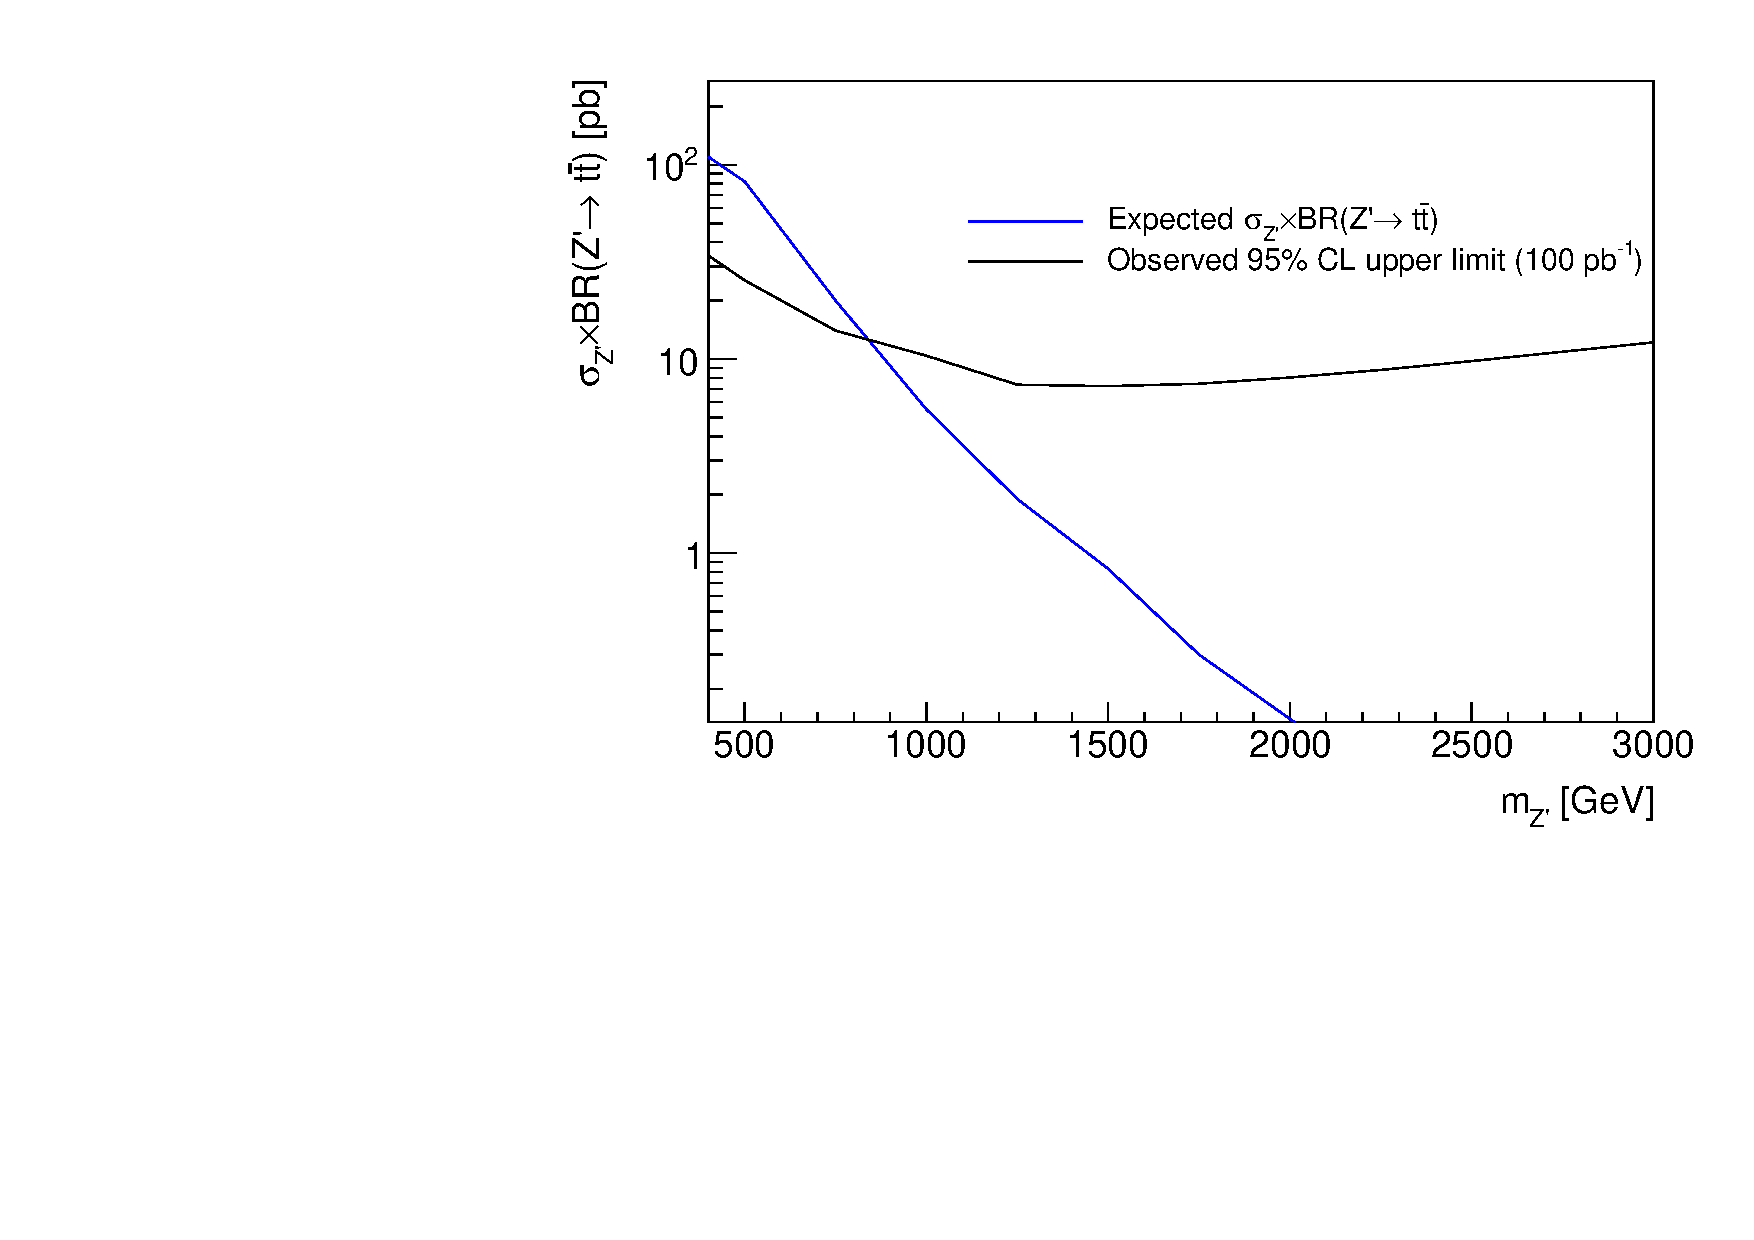
\includegraphics[width=\textwidth]{../pics/limits.pdf}
 \caption{Upper limits for $Z'$ cross section depending on the mass. The mass region below the point of intersect is excluded at 95\% CL.}
 \label{pic:limits}
\end{figure}
This shows a lower bound on the $Z'$ mass of around 850 GeV. 


% Notes:- 6.2c: some have fluctuations -> nothing to worry about. But in jet_eta, jet_pt and lep_eta for example the data points are almost always below the MC-expectation by fairly the same amount ->maybe there is a small, overall factor missing
% 	- 6.2d: from inv_massSys no Z' signal can be seen by eye.
% 	- 7.1a: from results/notes we get a p-value of 0.46. For 95 C.F. you get chi=36.4149 which means that the impact of the Z' cross section gets increased until this chi is reached.
% 	- 7.1d: by doing this, the lighter Z' overproduce the observed jets up to the mass of 850 GeV above which the Z' boson is still viable

\section{Conclusion}
The goal of this lab course was to look for BSM $t\bar t$ resonances in ATLAS data. Starting with preselected datasets, further selection conditions 
for the samples are posed. Such as the occurence of one reconstructed lepton to cover the decay topology with the best balance of emergence and
detectability. These conditions are also applied to MC simulations of significant background processes, most notably $t\bar t$. From the data and
the simulations the invariant mass of the system as derived quantitiy gets chosen to have the best discriminatory power as it shows a peak at 
the resonance of the applicable particle(s). Stacked plots of all background processes are made to identify a possible signal by comparison with
the data. Since no significant signal was found, a lower bound on the $Z'$ mass is set at around 850 GeV at 95\% CL.\\
\noindent This lab course is indeed an interesting process to understand the origin of physical constraints needed by theorists. Particularly the 
knowledge of the statistical analysis is an important gain.
Searching for $Z'$ signals is a major task nowadays. Depending on the chosen
model, however, the achieved lower bound here is already outdated and is set to 2-5 TeV \cite{Atlaslimits}\cite{pdg}\cite{1503.08929}.

\newpage
 \begin{thebibliography}{WissOnl}
 \bibitem{Atlas} ATLAS Collaboration, \textit{The ATLAS Experiment at the CERN Large Hadron Collider}, JINST 3 (2008) S08003
 \bibitem{etaNotch} ATLAS Collaboration, \textit{ATLAS Jet Trigger in the Early $\sqrt{s}$=7\,TeV Data}, ATLAS-CONF-2010-094, 2010. \href{https://cdsweb.cern.ch/record/1299109}{https://cdsweb.cern.ch/record/1299109}
 \bibitem{anl} S. Bartkowski, J. Erdmann, K. Kröninger, \textit{Lehrstuhlversuch ``Search for $t\bar t$ resonances with ATLAS data}, (2016), TU Dortmund
 \bibitem{Atlaslimits} ATLAS Collab., note ATLAS-CONF-2013-017, Mar. 2013.
 \bibitem{pdg}   C.~Patrignani {\it et al.} [Particle Data Group Collaboration],
 ``Review of Particle Physics,''
  Chin.\ Phys.\ C {\bf 40}, no. 10, 100001 (2016).
  doi:10.1088/1674-1137/40/10/100001
 \bibitem{1503.08929}  P.~Athron, D.~Harries and A.~G.~Williams,
  ``$Z'$ mass limits and the naturalness of supersymmetry,''
  Phys.\ Rev.\ D {\bf 91}, 115024 (2015)
  doi:10.1103/PhysRevD.91.115024
  [arXiv:1503.08929 [hep-ph]].
 \end{thebibliography}

% ========================================
%	Literaturverzeichnis
% ========================================

%\bibliographystyle{plainnat}			% Bibliographie-Style auswählen
%\bibliography{BIBDATEI}			% Literaturverzeichnis

% ========================================
%	Das Dokument endent
% ========================================
\end{document}
